\subsection{Protocol Description}

SAND (recursive acronym for \textit{SAND Anonymous Distribution}) is an
application layer network protocol on top of the TCP/IP stack. It makes use of a
worldwide P2P network to allow anonymously distributing files on the internet.

The participants in the network are:
\begin{itemize}
    \item Peers: Normal nodes which exchange files between them
    \item DNL Nodes: Nodes which serve the role of providing an initial set of 
neighbors for new peers. The addresses of these nodes should be publicly known.
DNL nodes share a distributed list of all the peers in the network between them,
which is periodically synchronized.
\end{itemize}

In this P2P network each node can act as proxy for another node to provide
anonymity in communication. The two parties which exchange a file between them
are completely unknown to each other. This is achieved by the means of a file
searching algorithm that recursively propagates a request through the network
while probing each node until the file is found.

SAND can additionally use UPnP to programmatically add a port mapping to the 
Internet Gateway Device. This will allow incoming messages on the port on which 
the client application is listening, if the device is sitting behind a NAT 
capable gateway. Other mechanisms for NAT traversal can be used as well, 
depending on the protocol implementation.

\subsection{Messages}

The protocol consists of a number of messages (also called requests), which may 
or may not receive a reply, depending on the type of the message. The request 
contains a 1-byte code which identifies the request type. The rest of the 
message is occupied by auxiliary data which are specific to each request type. 
The reply format is similar, but instead of a request code, it contains a 
1-byte status code. The status code can be interpreted in various ways, 
depending on the request type.

\begin{figure}[H]
    \centering
    \scalebox{.33}{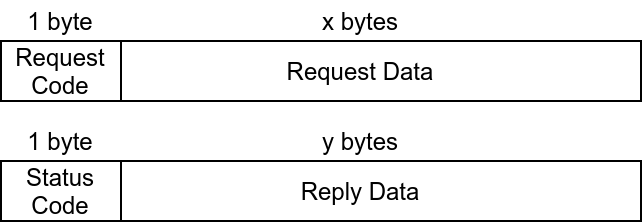
\includegraphics{figures/format}}
\end{figure}

Request codes are divided in 8 categories, each having 32 values:
\begin{itemize}
    \item Codes 0 - 31: Reserved / experimental
    \item Codes 32 - 63: Peer discovery
    \item Codes 64 - 95: File searching
    \item Codes 96 - 127: File transfer
    \item Codes 128 - 255 (4 categories): Unused
\end{itemize}

The following sections will present the main purpose and formats for the type of
messages exchanged between nodes. If the reply format is missing, then the reply
only contains the status code, unless specified otherwise. If the request format
is missing too, then the request only contains the request type.

\subsection{Status Codes}

The only status codes defined by the specification are:
\begin{itemize}
    \item 0 - Success
    \item 1 - Generic Error
\end{itemize}

Other status codes may be defined by implementations.
